% =============================================================================
%  UML 2.5 Activity Diagram: Single-objective Iterative Domain Contraction
%  Linear top-to-bottom main column; loop-back via the left margin.
%  Compile:  pdflatex fig_idc_activity_so.tex
% =============================================================================
\documentclass[border=4pt,tikz]{standalone}
\usetikzlibrary{positioning,shapes.geometric,shapes.misc,arrows.meta,calc,fit}

\begin{document}
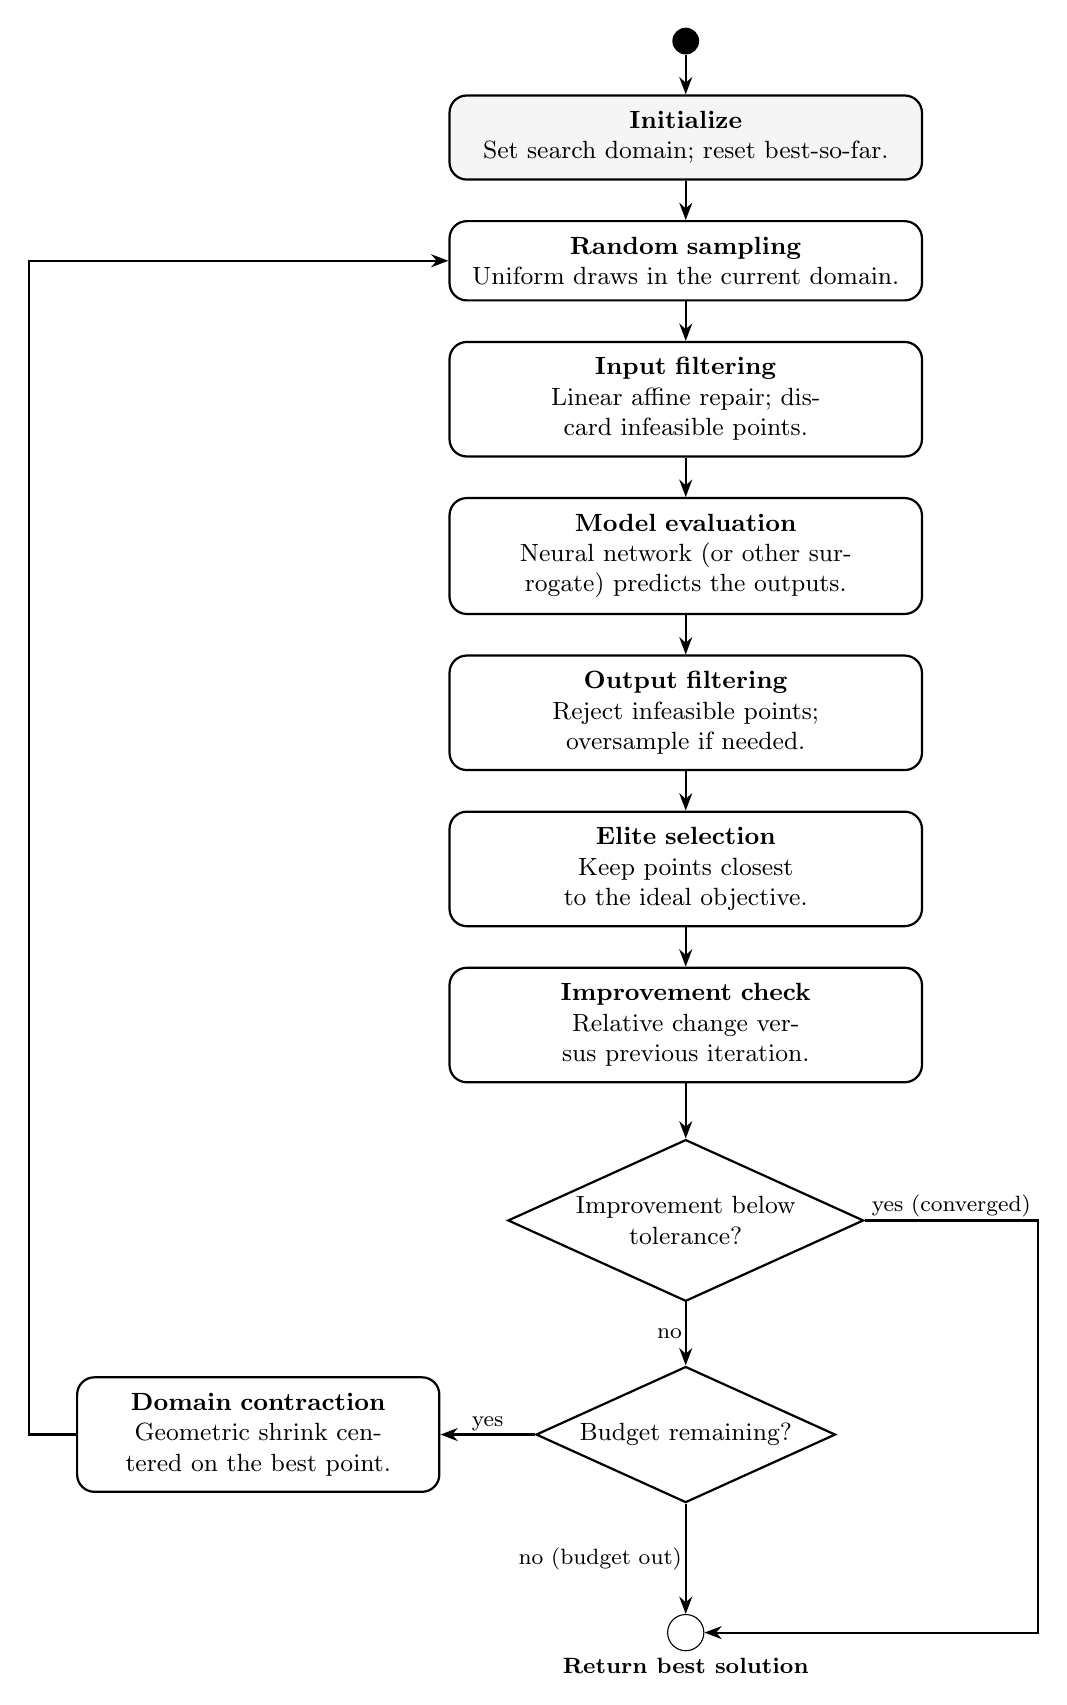
\begin{tikzpicture}[
    font=\small,
    >={Stealth[length=2.2mm]},
    node distance=5mm and 9mm,
    initial/.style   = {circle, fill=black, minimum size=3.4mm, inner sep=0pt},
    final/.style     = {circle, draw, minimum size=4.6mm, inner sep=0pt,
                        label={[anchor=center]center:{\large$\bullet$}}},
    action/.style    = {rectangle, rounded corners=2.2mm, draw, thick,
                        align=center, minimum height=8mm, minimum width=58mm,
                        inner sep=2.0mm, text width=56mm},
    sideaction/.style= {rectangle, rounded corners=2.2mm, draw, thick,
                        align=center, minimum height=8mm, minimum width=44mm,
                        inner sep=2.0mm, text width=42mm},
    init/.style      = {rectangle, rounded corners=2.2mm, draw, thick,
                        align=center, minimum height=8mm, minimum width=58mm,
                        inner sep=2.0mm, fill=black!4, text width=56mm},
    decision/.style  = {diamond, draw, thick, align=center, aspect=2.2,
                        inner sep=0.6mm, text width=28mm},
    flow/.style      = {-{Stealth[length=2.2mm]}, thick},
    label/.style     = {font=\footnotesize, inner sep=1pt}
]

% --- Main column (top to bottom) --------------------------------------------
\node[initial]                                  (start) {};
\node[init,    below=of start]                  (init)
  {\textbf{Initialize}\\
   Set search domain; reset best-so-far.};

\node[action,  below=of init]                   (random)
  {\textbf{Random sampling}\\
   Uniform draws in the current domain.};

\node[action,  below=of random]                 (inputf)
  {\textbf{Input filtering}\\
   Linear affine repair; discard infeasible points.};

\node[action,  below=of inputf]                 (eval)
  {\textbf{Model evaluation}\\
   Neural network (or other surrogate) predicts the outputs.};

\node[action,  below=of eval]                   (outf)
  {\textbf{Output filtering}\\
   Reject infeasible points; oversample if needed.};

\node[action,  below=of outf]                   (select)
  {\textbf{Elite selection}\\
   Keep points closest to the ideal objective.};

\node[action,  below=of select]                 (measure)
  {\textbf{Improvement check}\\
   Relative change versus previous iteration.};

\node[decision,below=7mm of measure]            (conv)
  {Improvement below\\ tolerance?};

\node[decision,below=8mm of conv]               (max)
  {Budget remaining?};

\node[final,   below=14mm of max]               (end) {};
\node[label,   below=0.5mm of end]              {\textbf{Return best solution}};

% --- Side branch (left): Domain contraction ---------------------------------
\node[sideaction, left=12mm of max]             (reshape)
  {\textbf{Domain contraction}\\
   Geometric shrink centered on the best point.};

% --- Flows -------------------------------------------------------------------
\draw[flow] (start)   -- (init);
\draw[flow] (init)    -- (random);
\draw[flow] (random)  -- (inputf);
\draw[flow] (inputf)  -- (eval);
\draw[flow] (eval)    -- (outf);
\draw[flow] (outf)    -- (select);
\draw[flow] (select)  -- (measure);
\draw[flow] (measure) -- (conv);

% Decisions: "no" labels on the LEFT
\draw[flow] (conv) -- node[label,left]{no} (max);
\draw[flow] (max)  -- node[label,left]{no (budget out)} (end);

% Termination from convergence: bend RIGHT, drop down, enter end from the east
\draw[flow] (conv.east) -- node[label,above]{yes (converged)}
           ++(22mm,0) |- (end.east);

% Loop-back: D2.west -> reshape (left), then up the left margin to random.west
\draw[flow] (max.west) -- node[label,above]{yes} (reshape.east);
\draw[flow] (reshape.west) -- ++(-6mm,0) |- (random.west);

\end{tikzpicture}
\end{document}
